\paragraph{Model-dependent limits}
\label{sec:model_dep}
%
At the tree level, the Higgs sector of the MSSM can be specified by suitable choices for two variables, 
often chosen to be the mass $m_{\PA}$ of the pseudoscalar Higgs boson
and $\tan\beta$, the ratio of the \mbox{vacuum} expectation
values of the two Higgs doublets.
The typically large radiative corrections are 
fixed based on experimentally and phenomenologically sensible choices for
the supersymmetric parameters, each choice defining a particular benchmark scenario~\cite{Carena:2013ytb}.
Generally, MSSM scenarios assume that the 125 GeV Higgs boson is the lighter scalar \Ph, 
an assumption that is compatible with the current experimental constraints 
for at least a significant portion of the $m_{\PA}$--$\tan\beta$ parameter space.
The di-tau lepton final state provides the most sensitive direct search for additional
Higgs bosons predicted by the MSSM for intermediate and high values of tan$\beta$, 
because of the enhanced
coupling to down-type fermions.
%
\begin{figure}[htbp]
\begin{center}
\subfloat[$\mhmodp$]{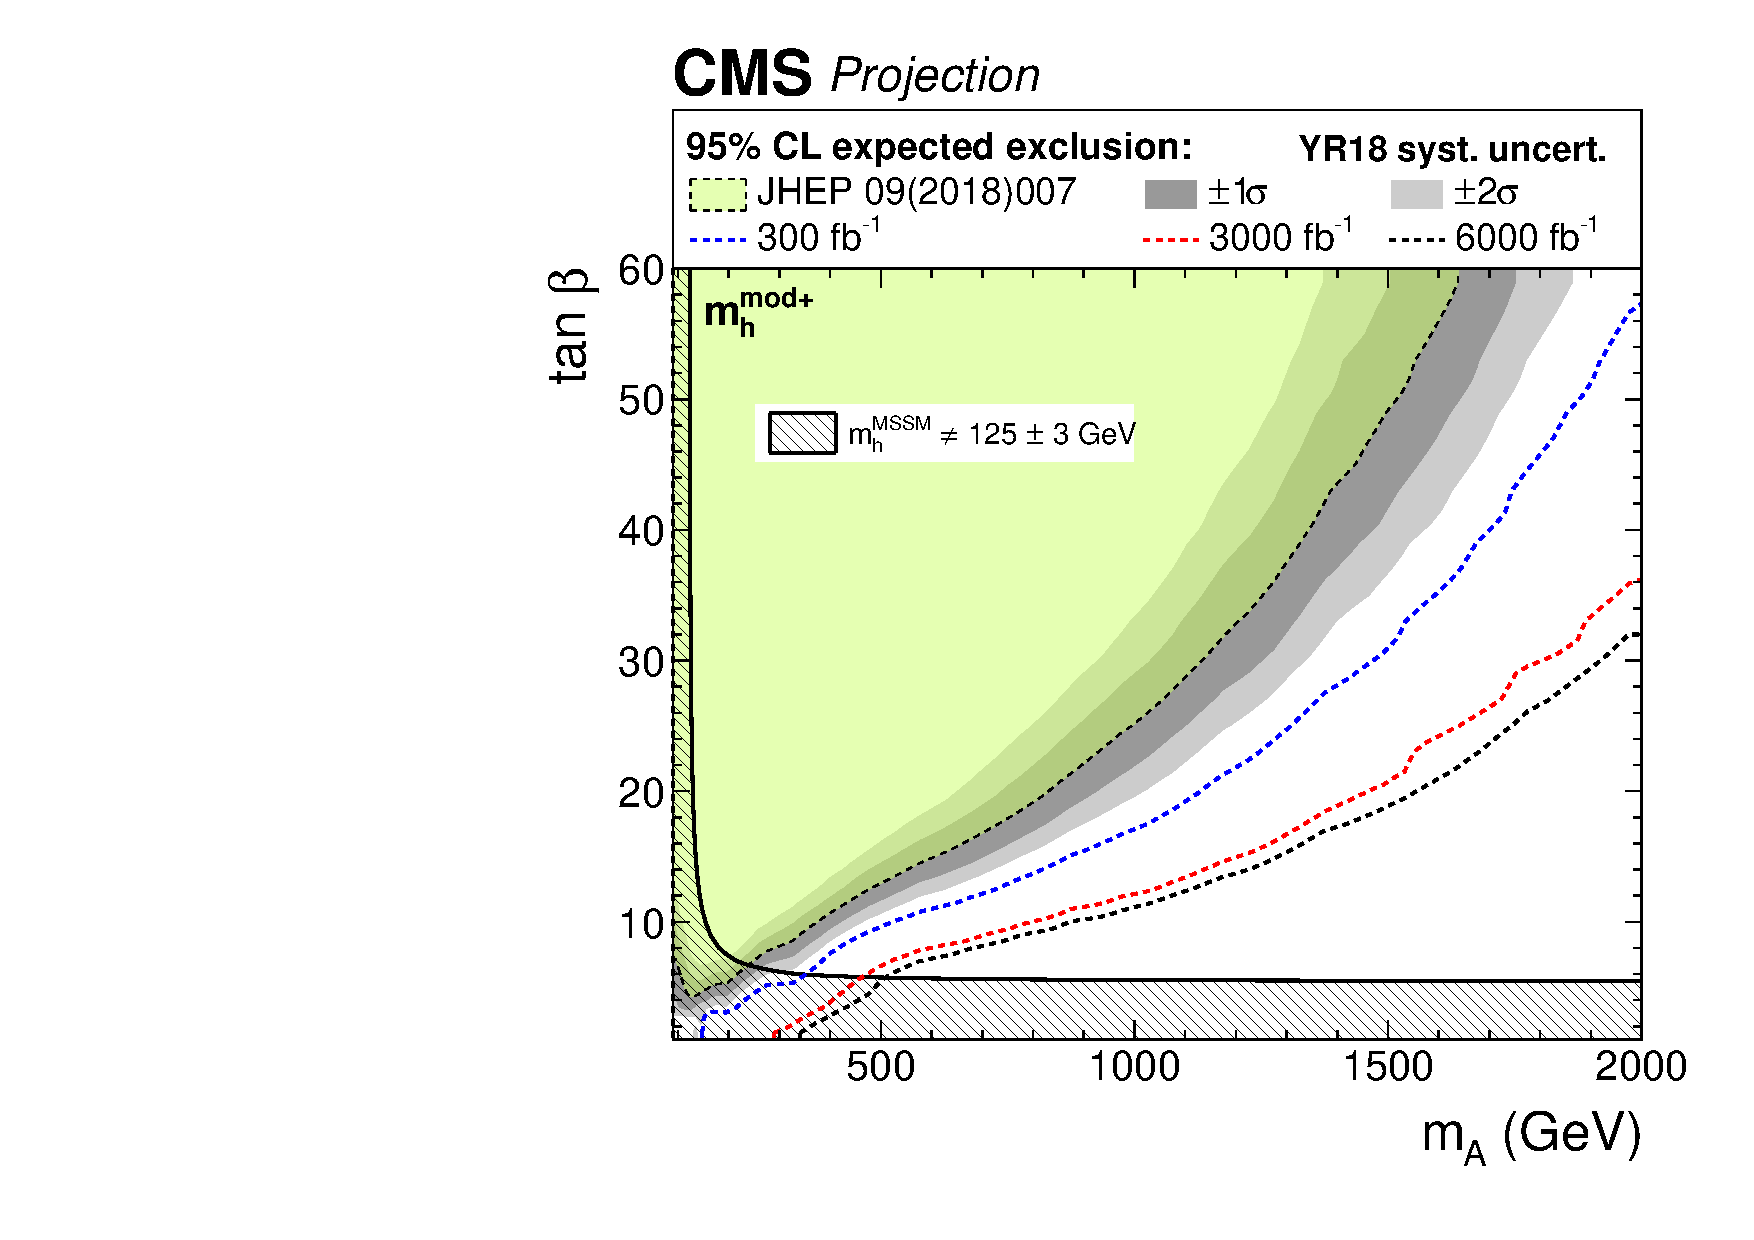
\includegraphics[width=0.6\textwidth]{\main/section9/cms_htt/figures/mssm_mhmod_jul31_scen2_pas.pdf}}\\
\subfloat[hMSSM]{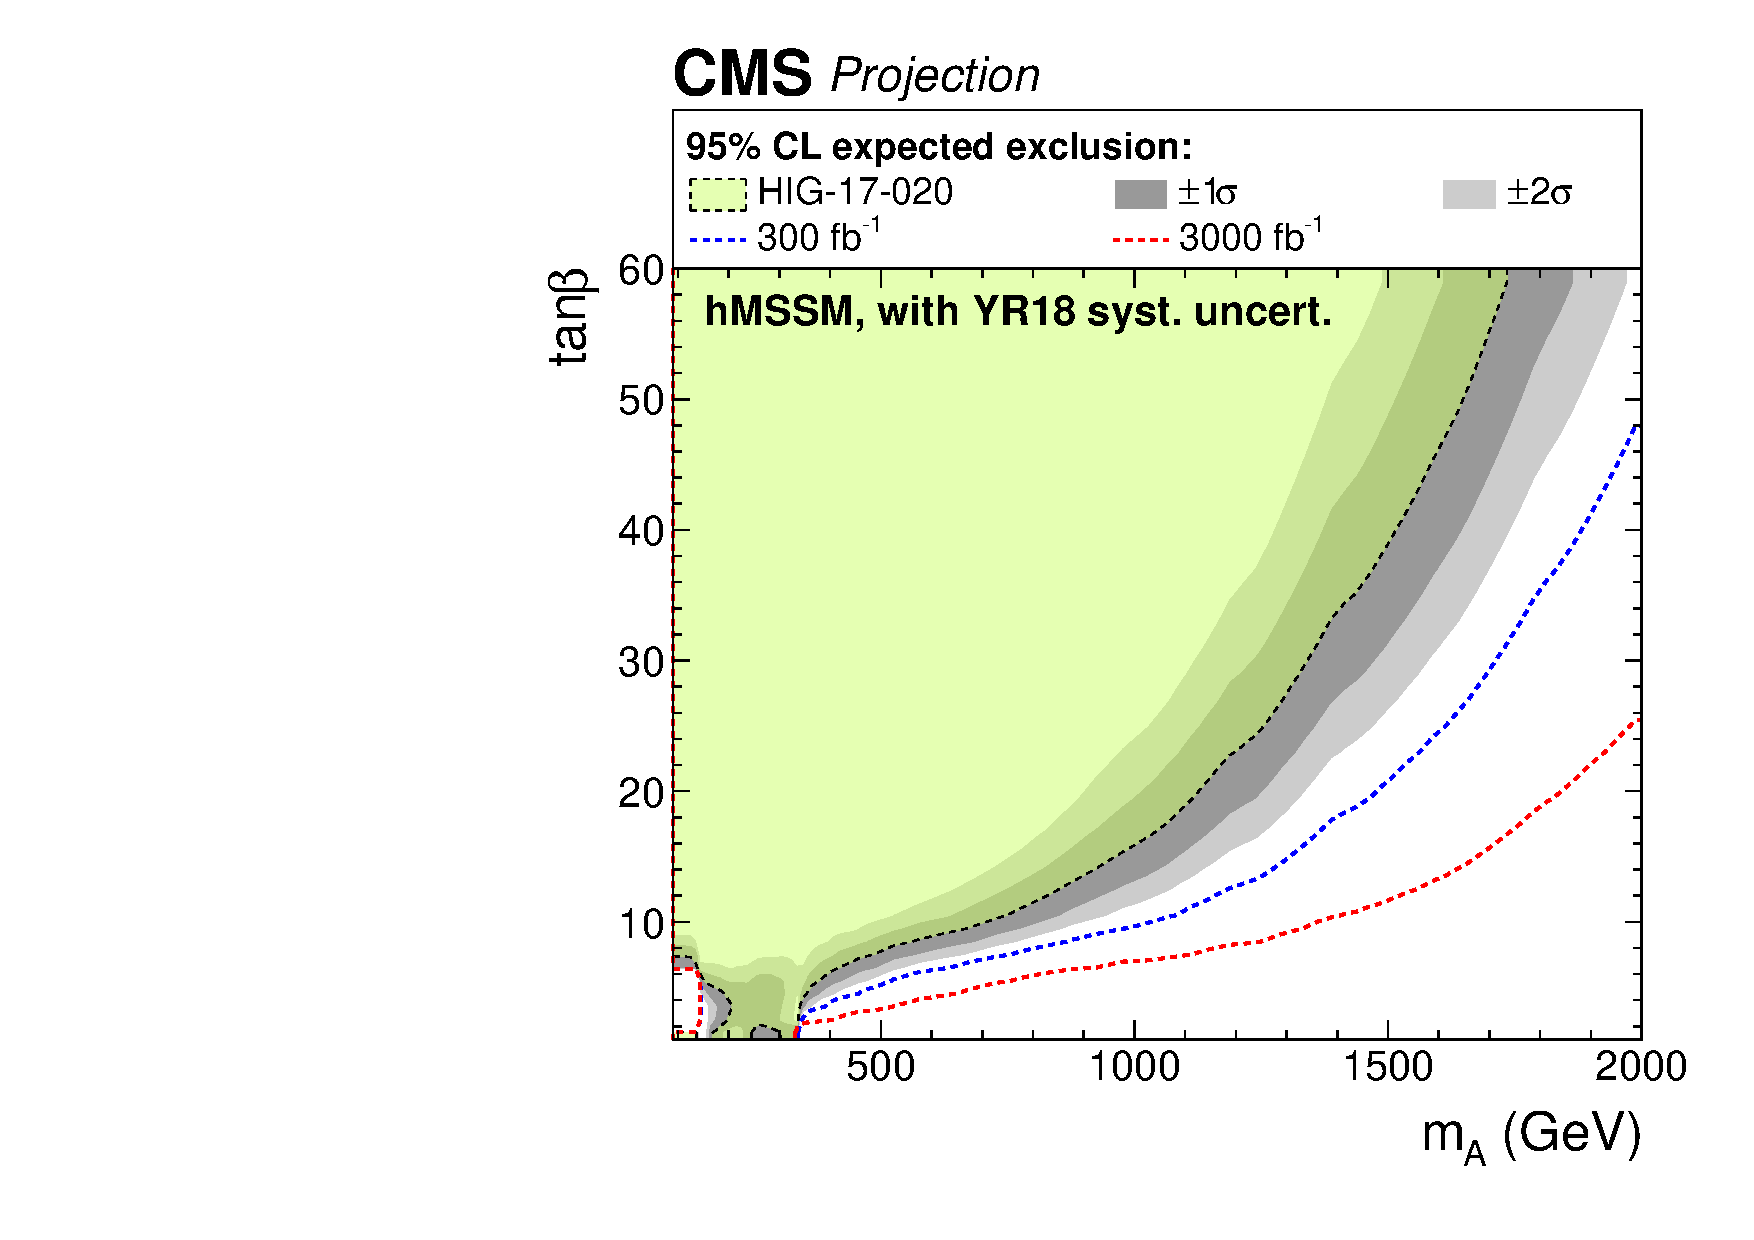
\includegraphics[width=0.45\textwidth]{\main/section9/cms_htt/figures/mssm_hmssm_jul31_scen2_pas.pdf}}
\subfloat[tau-phobic]{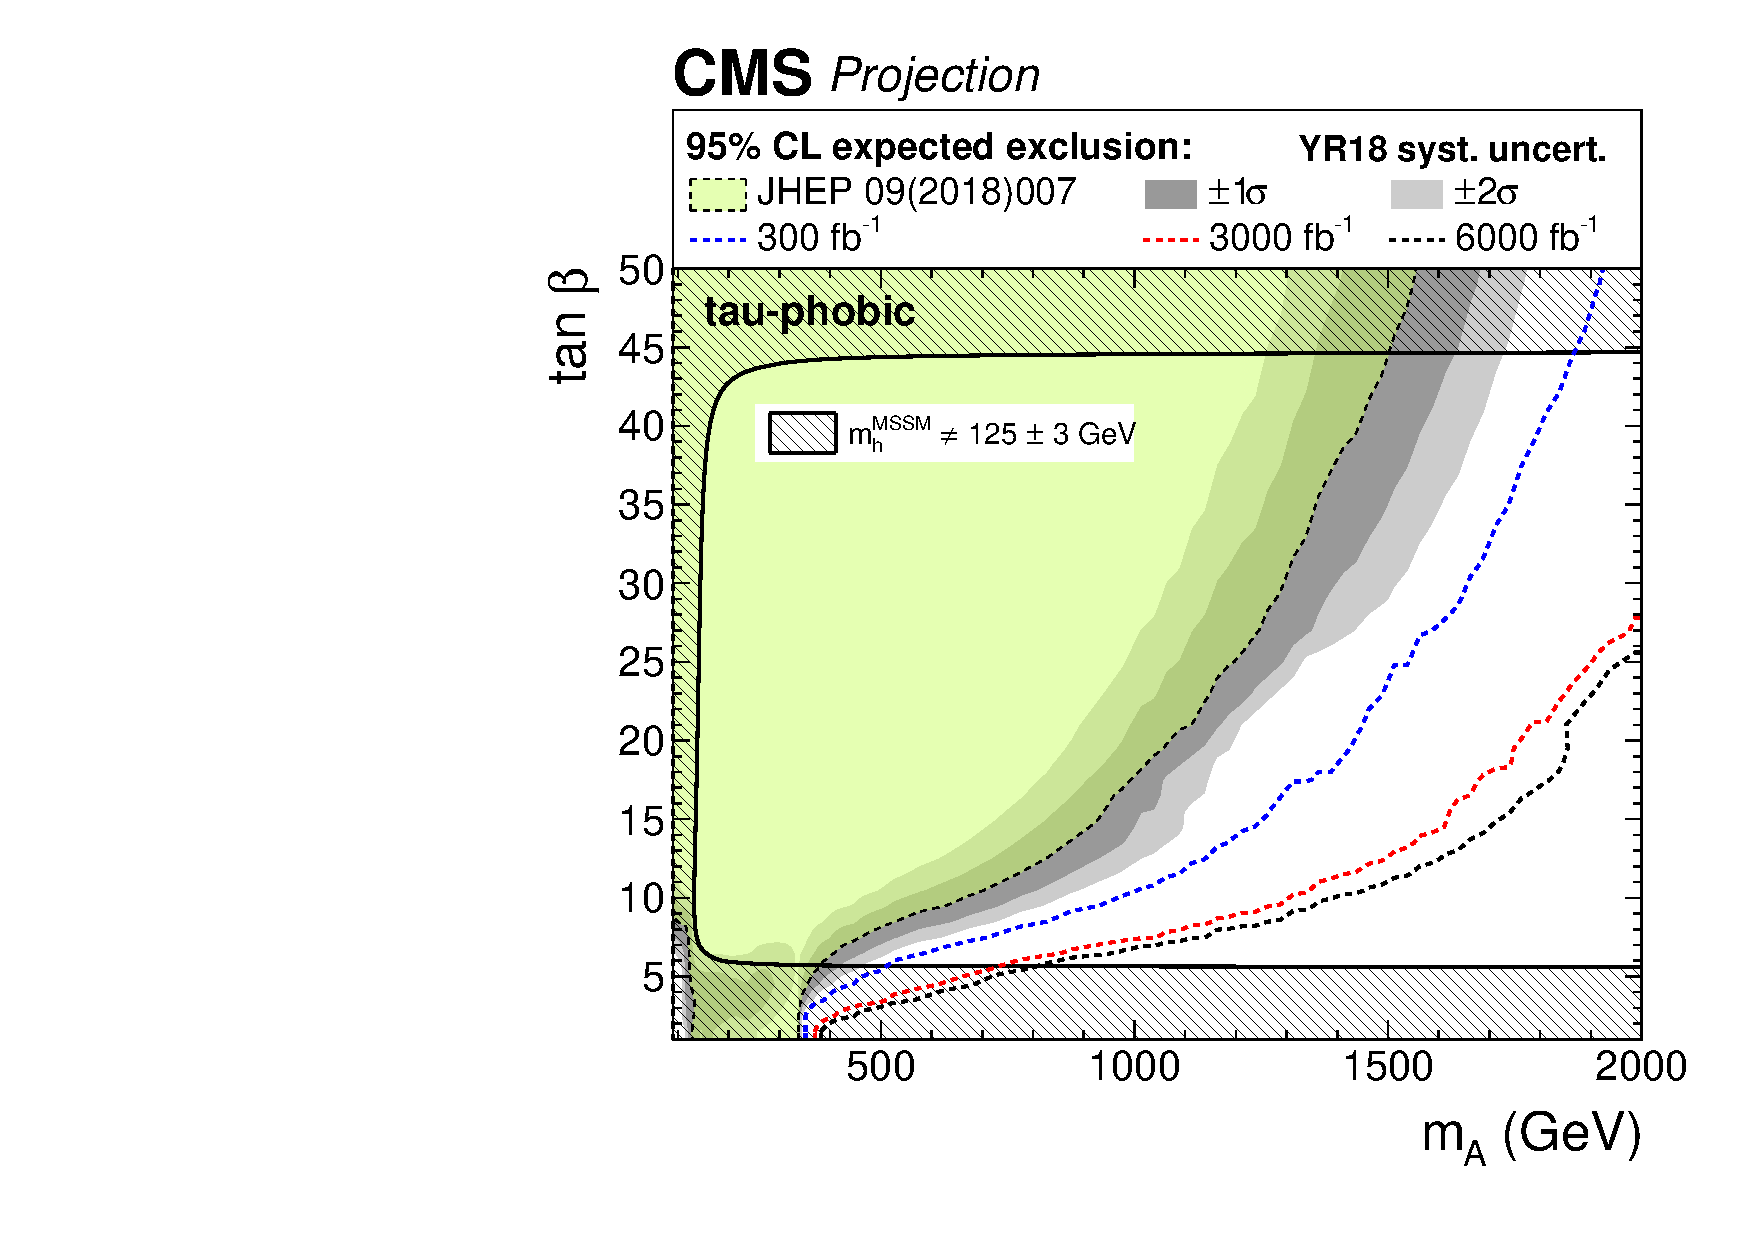
\includegraphics[width=0.45\textwidth]{\main/section9/cms_htt/figures/mssm_tauphobic_aug03_scen2_pas.pdf}}
\end{center}
\caption{Projection of expected MSSM \htt 95\% CL upper limits based on 2016 data~\cite{HIG-17-020} for different benchmark 
scenarios, with YR18 systematic uncertainties. The limit shown for 6000\fbinv is an approximation of the sensitivity with 
the complete HL-LHC dataset to be collected by the ATLAS and CMS experiments, corresponding to an integrated luminosity of 3000\fbinv each. 
The limits are compared to the CMS result using 2016 data~\cite{HIG-17-020}; for the tau-phobic scenario, 
it is a new interpretation of the information given in this reference. 
}
\label{fig:model_mssm1}
\end{figure}

The analysis results are interpreted in terms of these benchmark scenarios based on the profile likelihood ratio of the 
background-only and the tested signal-plus-background hypotheses. 
For this purpose, the predictions from both production modes and both heavy neutral Higgs bosons are combined.
Figure~\ref{fig:model_mssm1} shows the results 
for three different benchmark scenarios:
the $\mhmodp$, the hMSSM, and the tau-phobic scenarios~\cite{HIG-17-020}.
The sensitivity reaches up to Higgs boson masses
of 2 TeV for values of $\tan \beta$ of 36, 26, and 28
for the $\mhmodp$, the hMSSM, and the tau-phobic scenarios,
respectively.
Even at low mass, improvements are expected but in this case they are mostly 
a consequence of reduced systematic uncertainties and not 
the additional data in the signal region.